\documentclass{beamer}
%
% Choose how your presentation looks.
%
% For more themes, color themes and font themes, see:
% http://deic.uab.es/~iblanes/beamer_gallery/index_by_theme.html
%
\mode<presentation>
{
  \usetheme{CambridgeUS}      % or try Darmstadt, Madrid, Warsaw, ...
  \usecolortheme{default} % or try albatross, beaver, crane, ...
  \usefonttheme{default}  % or try serif, structurebold, ...
  \setbeamertemplate{navigation symbols}{}
  \setbeamertemplate{caption}[numbered]
} 

\usepackage[english]{babel}
\usepackage[utf8x]{inputenc}

\title[Open Source Workshop (beamer)]{Linux install Party}
\author[Elsa, Pablo]{Elsa Guillot, Pablo Hernandez}
\institute[IFS]{IFS, Massey University}
\date{19/10/14}

\begin{document}

\begin{frame}
  \titlepage
%  \includegraphics{Fussta.png}
%    \includegraphics{Messa.png}
%      \includegraphics{McDiarmid.png}
%            \includegraphics{Opensources.png}	
\end{frame}

% Uncomment these lines for an automatically generated outline.
\begin{frame}{Outline}
  \tableofcontents
\end{frame}

\section{Linux Install Party}
\begin{frame}
\frametitle{Welcome!}
\begin{itemize}
\item Internet \textbf{MUevents}, password \textbf{Op3nSourc3}
\item Tea offered by FUSSTA
\item BBQ tonight 85 Campbell Street, offered by MESA
\item You will each receive a Linux Mint Install CD
\end{itemize}
\end{frame}

\subsection{An OS story}
\begin{frame}
\frametitle{OS and Russian dolls}
\begin{itemize}
  \item Operating System: Windows XP, Mac, Linux Ubuntu, DOS
  \item Most computer run under a unique OS
  \item Dual boot: you chose at the start which OS you run
  \item Virtual Machine: an OS within an other OS
\end{itemize}
\end{frame}

\begin{frame}
\frametitle{OS}
\begin{tabular}{|ccc|}
\hline
Windows & Mac (OsX) & Linux\\
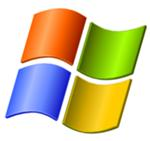
\includegraphics[scale=0.2]{windows.jpg} & 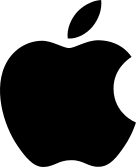
\includegraphics[scale=0.2]{apple.png} & 
\includegraphics[scale=0.2]{mint.png}\\

\hline
Expensive & Expensive & Free (or not)\\
\multicolumn{2}{|c}{Close system/black box} & Open source\\
\multicolumn{2}{|c}{Limited control (data/system)} & Full control \\
Viruses &  \multicolumn{2}{c}{more secure}\\
Microsoft Office & Microsoft Office & LibreOffice \\
few distro & few distro & many distro\\
\multicolumn{2}{|c}{Hard to break} & Easy to break\\
\multicolumn{2}{|c}{Hard to fix} & Easy to fix\\
\multicolumn{2}{|c}{Professional support} & Community support \\
- & \multicolumn{2}{c|}{clear separation on admnistrative task}\\
\hline

\end{tabular}
\end{frame}


\begin{frame}{Dual Boot VS Virtual Machine}
\begin{columns}
\begin{column}{6cm}
\begin{center}
Virtual Box
\end{center}
\begin{itemize}
\item Easy to install / re-install
\item Safe for you data and your system
\item Good to test/ play around different OS
\item Require a big machine to run a smooth VB
\item You are still running windows underneath
\item Temporary solution
\end{itemize}
\end{column}
\begin{column}{6cm}
\begin{center}
Dual Boot
\end{center}
\begin{itemize}
\item Once install run Windows / Linux independently
\item Harder to install
\item High risk of data/system loss
\item Smoother to run
\item Can boost up your old computer
\item Long term solution
\end{itemize}
\end{column}
\end{columns}
\end{frame}

\subsection{Linux}
\begin{frame}
\frametitle{Linux-GNU}
\begin{columns}
\begin{column}{7cm}
\begin{itemize}
\item Linux is a UNIX-like system
\item Created by Linux Torvalds in 1991
\item The GNU project was created by Richard Stallman in 1993
\item Linux is developed independently by many entities, creating many distribution
\item They all share core concept
\end{itemize}
\end{column}
\begin{column}{4cm}
\begin{figure}

\includegraphics[scale=0.2]{ubuntu.png}\\%hspace{5mm}

\includegraphics[scale=0.2]{lubuntu.png}\\%hspace{5mm}

\includegraphics[scale=0.2]{kubuntu.png}\\

\includegraphics[scale=0.2]{mint.png}\\%hspace{5mm}

\includegraphics[scale=0.2]{debian.png}\\

\includegraphics[scale=0.2]{fedora.png}\\%hspace{5mm}

\includegraphics[scale=0.2]{redhat.png}\\%hspace{5mm}

\includegraphics[scale=0.2]{centos.png}\\

\includegraphics[scale=0.2]{arch.png}\\%hspace{5mm}

\includegraphics[scale=0.2]{suse.png}
%
\includegraphics[scale=0.1]{mageia.png}
\end{figure}
\end{column}
\end{columns}
\end{frame}
\begin{frame}
\frametitle{Distributions}
\begin{columns}
\begin{column}{10cm}
\begin{itemize}
\item To switch from one distribution to another you must re-install the whole system
\item They look different and have different applications already installed
\item Distributions target different uses
\item \textbf{Ubuntu} is the most user-friendly and popular
\item \textbf{Mint} is a user-friendly distro growing very fast
\item \textbf{Fedora} is popular among scientist and programmers
\item \textbf{RedHat} is a commercial distribution of Linux (sold to companies and come with support)
\item Some distribution are only for professional IT administrators
\item \textbf{You can give a try to different distribution with live CDs}
\end{itemize}
\end{column}
\begin{column}{1cm}
\begin{figure}

\includegraphics[scale=0.2]{ubuntu.png}\\%hspace{5mm}

\includegraphics[scale=0.2]{lubuntu.png}\\%space{5mm}

\includegraphics[scale=0.2]{kubuntu.png}\\

\includegraphics[scale=0.2]{mint.png}\\%hspace{5mm}

\includegraphics[scale=0.2]{debian.png}\\fa

\includegraphics[scale=0.2]{fedora.png}\\%hspace{5mm}

\includegraphics[scale=0.2]{redhat.png}\\%hspace{5mm}

\includegraphics[scale=0.2]{centos.png}\\

\includegraphics[scale=0.2]{arch.png}\\%hspace{5mm}

\includegraphics[scale=0.2]{suse.png}\\%hspace{5mm}
%
\includegraphics[scale=0.1]{mageia.png}
\end{figure}
\end{column}
\end{columns}
\end{frame}

\begin{frame}
\frametitle{Linux Mint}
\begin{figure}
\begin{center}

\includegraphics[scale=0.5]{mint.png}\\%hspace{5mm}
\end{center}
\end{figure}
\begin{itemize}
\item We will install Mint 
\item Very popular at the moment
\item Good support community on the internet
\item Easy to use
\item Easy transition from other OS to Mint
\item It looks a little like Windows
\end{itemize}
\end{frame}

\begin{frame}
\frametitle{Linux 101 (Mint)}
\begin{itemize}
\item It has already most software install
\item Firefox, vlc 
\item No Word, but Libre Office instead
\item Navigate as you would with Windows / Mac
\item Its Desktop Environment is called \textbf{Cinnamon}
\end{itemize}
\end{frame}


\begin{frame}
\frametitle{Linux Desktop Environment}
\begin{itemize}
\item The DE is your interface with the Linux system
\item The way things look, the shortcuts you have, how you launch programs
\item You can install an other DE \textbf{without} reinstalling the system
\item Example of other DE: Gnome, Unity, KDE
\item DE are more or less dependent on Distributions
\end{itemize}
\end{frame}


\begin{frame}
\frametitle{Linux 101 (Mint)}
\begin{itemize}
\item Start application via the menu 
\item Or launch any program with Alt+F2 and enter the name of the program
\item Switch between windows with Alt+Tab
\item You have several Workspaces
\item Console interface : ctrl+Alt+T
\end{itemize}
\end{frame}

\begin{frame}
\frametitle{Linux 101 (Mint) - console}
\begin{tabular}{|l|l|}
\hline
command & action \\
\hline
ls & shows where you are \\
cd \textit{directory}& change directory, i.e. move\\
cp \textit{oldfile newfile} & copy (file) \\
cp -r \textit{oldirectory newdirectory}& copy directory\\
mkdir \textit{}& make directory\\
less \textit{file}& show content of file \\
wget \textit{url} & download internet page \\
ls & list the files in the current directory\\
\textit{programname} & launch the program\\
\hline
\end{tabular}
\end{frame}

\section{Open Source}

\begin{frame}
\frametitle{What is open Source}
\begin{itemize}
\item All programs are released under a license, which allows different access and use of the program
\item A program is open source if it is possible to access its code source, i.e. the recipe of how it works to anyone
\item Open source does not mean free (depending on definition)
\item Open source program should be modifiable by anyone 
\item GNU Linux is an open source project
\item We will focus on project being free and open source, as promoted by the open source initiative
\item The definition of open source by the OSI can be found here \url{opensource.org/docs/osd}
\end{itemize}
\end{frame}

\begin{frame}
\frametitle{Why should a program be open source}
\begin{itemize}
\item Allows a better usage 
\item Better control of what the program is doing
\item Permits continuous improvement
\item Easier to fix if it does not work
\item Less dependent on a single entity for support
\item Like science, IT builds up on previous work to make bigger things
\end{itemize}
\end{frame}

\begin{frame}
\frametitle{Open source examples}
\begin{itemize}
\item LibreOffice (alternative to Microsoft Office suit)
\item Mozilla Firefox 
\item Mozilla Thunderbird (email interface)
\item Android
\item GNU Octave (alternative to Matlab)
\item Git
\item Zotero
\end{itemize}
\end{frame}


\section{Zotero}
\begin{frame}
\frametitle{Zotero}
\begin{itemize}
\item Zotero is a \textbf{free open source} alternative to EndNotes and Mendeley
\item Getting more and more popular
\item Easy to use
\item Easy to install
\item \textbf{Synchronize} you library on different computers
\item Plugin to your web-browser
\item Compatible with latex
\item Intergration with Word, OpenOffice, LibreOffice
\end{itemize}
\end{frame}

\section{Github}
\begin{frame}
\frametitle{Git}
\begin{itemize}
\item Versionning software
\item Alternative to svn
\item Saves you work, along with old versions
\item Enable several people working on the same project
\item Decentralize the copies of your project
\end{itemize}
\end{frame}


\begin{frame}
\frametitle{Github}
\begin{itemize}
\item 
\item 
\item 
\item 
\item 
\item 
\item 
\item 
\end{itemize}
\end{frame}


\end{document}
